\documentclass[12pt,letterpaper]{article}
\usepackage[utf8]{inputenc}
\usepackage[spanish]{babel}
\usepackage{graphicx}
\usepackage[left=2cm,right=2cm,top=2cm,bottom=2cm]{geometry}
\usepackage{graphicx} % figuras
% \usepackage{subfigure} % subfiguras
\usepackage{float} % para usar [H]
\usepackage{amsmath}
%\usepackage{txfonts}
\usepackage{stackrel} 
\usepackage{multirow}
\usepackage{enumerate} % enumerados
\renewcommand{\labelitemi}{$-$}
\renewcommand{\labelitemii}{$\cdot$}
% \author{}
% \title{Caratula}
\begin{document}

% Fancy Header and Footer
% \usepackage{fancyhdr}
% \pagestyle{fancy}
% \cfoot{}
% \rfoot{\thepage}
%

% \usepackage[hidelinks]{hyperref} % CREA HYPERVINCULOS EN INDICE

% \author{}
\title{Caratula}

\begin{titlepage}
\begin{center}
\large{UNIVERSIDAD PRIVADA-DE-TACNA}\\
\vspace*{-0.025in}
\begin{figure}[htb]
\begin{center}

\includegraphics[width=8cm]{./Imagenes/logo}
\end{center}
\end{figure}
\vspace*{0.15in}
INGENIERIA DE SISTEMAS  \\

\vspace*{0.5in}
\begin{large}
TITULO:\\
\end{large}

\vspace*{0.1in}
\begin{Large}
\textbf{LABORATORIO ENCARGADO No 04} \\
\end{Large}

\vspace*{0.3in}
\begin{Large}
\textbf{CURSO:} \\
\end{Large}

\vspace*{0.1in}
\begin{large}
INTELIGENCIA DE NEGOCIOS\\
\end{large}

\vspace*{0.3in}
\begin{Large}
\textbf{DOCENTE(ING):} \\
\end{Large}

\vspace*{0.1in}
\begin{large}
 Patrick Cuadros Quiroga\\
\end{large}

\vspace*{0.2in}
\vspace*{0.1in}
\begin{large}
Integrantes: \\
\begin{flushleft}

Condori Choquecota, Jose Luis       \hfill	(2014049088) \\


\end{flushleft}
\end{large}
\end{center}

\end{titlepage}


\tableofcontents % INDICE
\thispagestyle{empty} % INDICE SIN NUMERO
\newpage
\setcounter{page}{1} % REINICIAR CONTADOR DE PAGINAS DESPUES DEL INDICE

\section{¿Que son los modelos dimensionales?} 
El modelado dimensional reside en la evidente simplicidad de los modelos y en la forma natural que la gente de negocios y la gente técnica puedan entender lo que significan estos modelos.
\\

Los modelos dimensionales tienen dos expresiones diferentes, lógica y física. La expresión puramente lógica queda plasmada en el siguiente diagrama.
\\
\\
	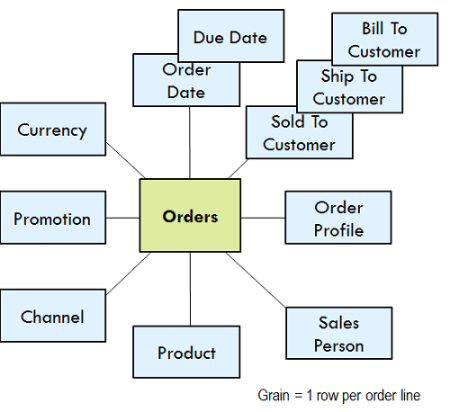
\includegraphics[width=7cm]{./Imagenes/dimensional} 

El diagrama del modelo lógico se transformará con bastante rapidez a un diseño técnico más específico repleto de nombres de tablas, nombres de campos, y declaraciones de claves primarias y foráneas.
\\
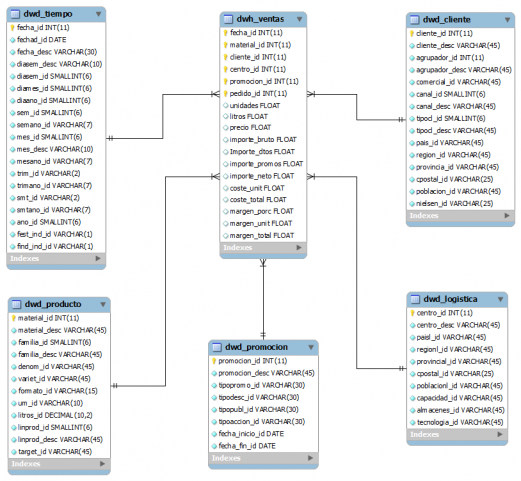
\includegraphics[width=7cm]{./Imagenes/fisica} 
\\
Recuperado de: datawarehouse.es

\section{Diagramas Dimensionales} 

\begin{itemize}
	\item Diagrama dimensional del ejercicio 1
	\\
	\begin{center}
	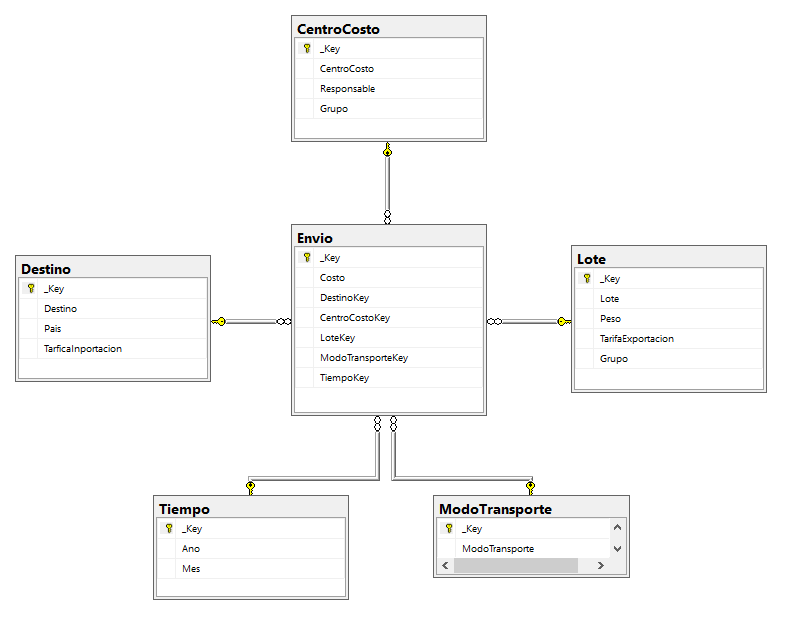
\includegraphics[width=13cm]{./Imagenes/md_ejer1} 
	\end{center}



\end{itemize} 
\section{Diagramas Dimensionales} 

\begin{itemize}
	\item Diagrama dimensional del ejercicio 2
	\\
	\begin{center}
	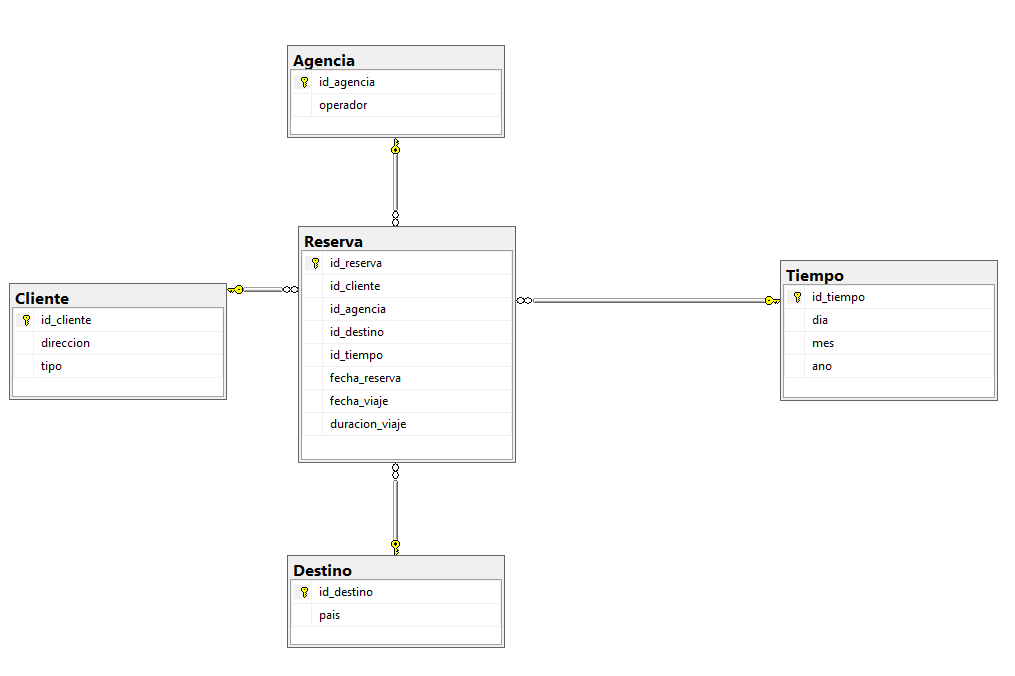
\includegraphics[width=13cm]{./Imagenes/md_ejer2} 
	\end{center}



\end{itemize} 
\section{Diagramas Dimensionales} 

\begin{itemize}
	\item Diagrama dimensional del ejercicio 3
	\\
	\begin{center}
	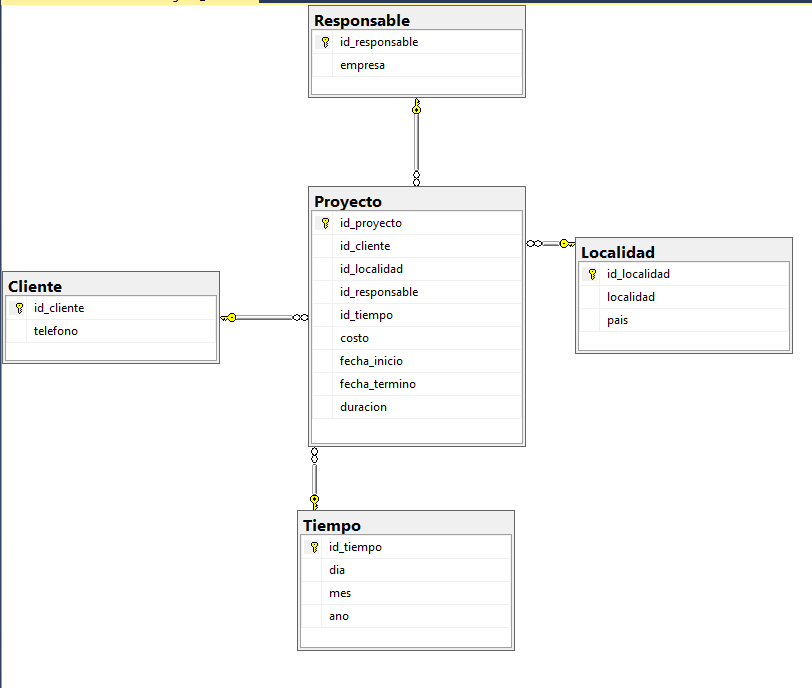
\includegraphics[width=13cm]{./Imagenes/md_ejer3} 
	\end{center}



\end{itemize} 
\section{Diagramas fisico} 

\begin{itemize}
	\item Diagrama fisico del ejercicio 1
	\\
	\begin{center}
	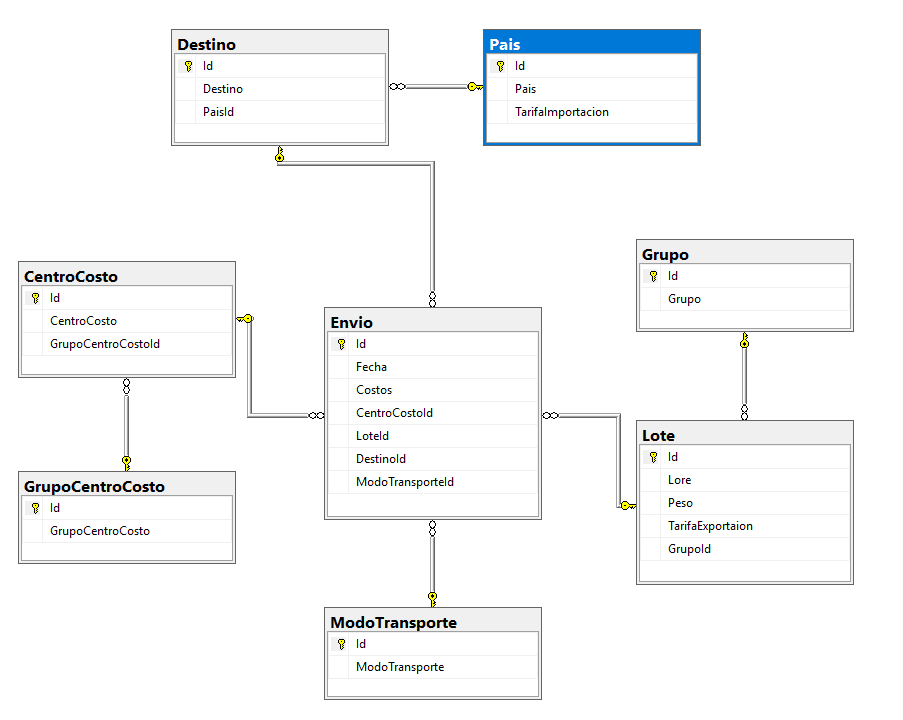
\includegraphics[width=13cm]{./Imagenes/mf_ejer1} 
	\end{center}



\end{itemize} 
\section{Diagramas fisico} 

\begin{itemize}
	\item Diagrama fisico del ejercicio 2
	\\
	\begin{center}
	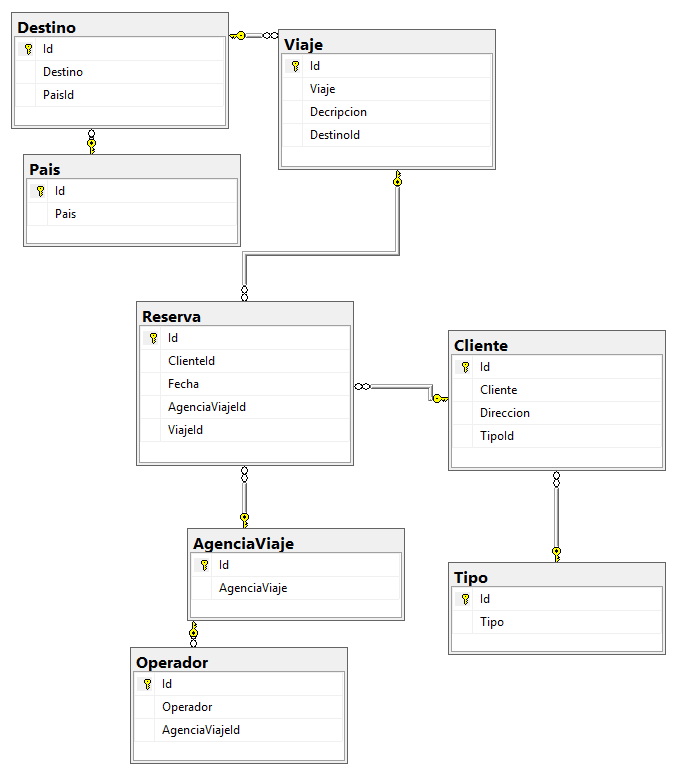
\includegraphics[width=13cm]{./Imagenes/mf_ejer2} 
	\end{center}



\end{itemize} 
\section{Diagramas fisico} 

\begin{itemize}
	\item Diagrama fisico del ejercicio 3
	\\
	\begin{center}
	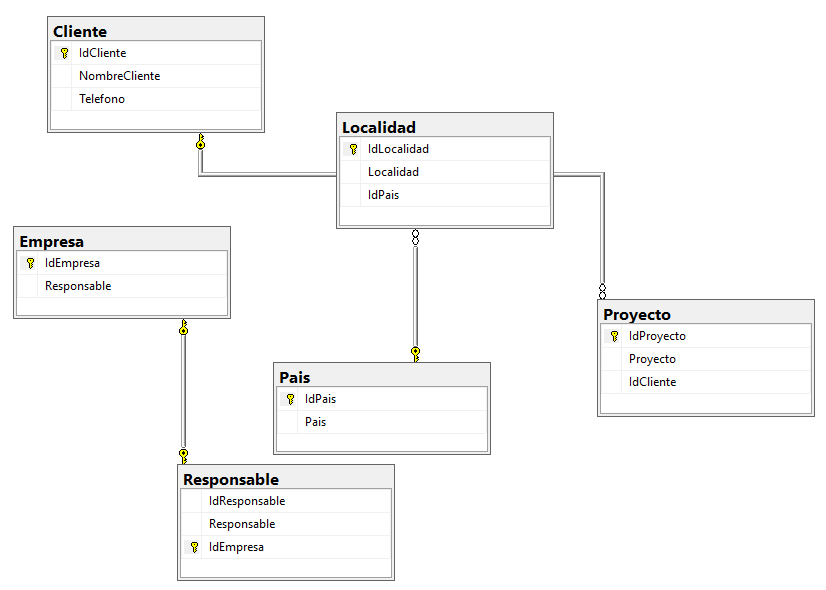
\includegraphics[width=13cm]{./Imagenes/mf_ejer3} 
	\end{center}



\end{itemize} 

\end{document}
